\begin{center}
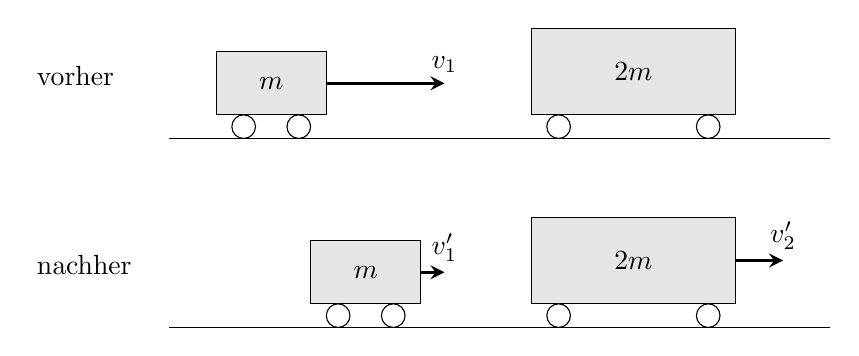
\begin{tikzpicture}[>=stealth]
 \node[anchor=west] at (0,0.8) {vorher};
 \draw (1.8,0) -- (10.2,0);
 \draw[fill=gray!20] (2.4,0.3) rectangle (3.8,1.1);
 \node at (3.1,0.7) {$m$};
 \draw[fill=white] (2.75,0.15) circle (0.15) (3.45,0.15) circle (0.15);
 \draw[->, very thick] (3.8,0.7) -- (5.3,0.7) node[above] {$v_1$};
 \draw[fill=gray!20] (6.4,0.3) rectangle (9,1.4);
 \node at (7.7,0.85) {$2m$};
 \draw[fill=white] (6.75,0.15) circle (0.15) (8.65,0.15) circle (0.15);
 \node[anchor=west] at (0,-1.6) {nachher};
 \draw (1.8,-2.4) -- (10.2,-2.4);
 \draw[fill=gray!20] (3.6,-2.1) rectangle (5,-1.3);
 \node at (4.3,-1.7) {$m$};
 \draw[fill=white] (3.95,-2.25) circle (0.15) (4.65,-2.25) circle (0.15);
 \draw[->, very thick] (5,-1.7) -- (5.3,-1.7) node[above] {$v_1'$};
 \draw[fill=gray!20] (6.4,-2.1) rectangle (9,-1);
 \node at (7.7,-1.55) {$2m$};
 \draw[fill=white] (6.75,-2.25) circle (0.15) (8.65,-2.25) circle (0.15);
 \draw[->, very thick] (9,-1.55) -- (9.6,-1.55) node[above] {$v_2'$};
\end{tikzpicture}
\end{center}

Der Gesamtimpuls bleibt erhalten:
\begin{align}
 m\,v_1 &= m\,v_1' + 2m\,v_2'
\end{align}
Die Masse $m$ kürzt sich heraus, und es folgt
\begin{align}
 v_2' &= \vZeF = \frac{\vEa-\vEe}{2} = \vZe \approx \result{\vZeP{0}{2}}
\end{align}
